This appendix holds the descriptive pass that precedes the Bayesian analysis.\footnote{The sweep is implemented in the notebook \href{https://github.com/FedericoSabbadini/patchAliasing/blob/main/notebooks/signal_analysis/appendix_reconstruction.ipynb}{\texttt{appendix\_reconstruction.ipynb}}.} It covers the fifteen geometries of \autoref{tab:hfModels}, five to a figure, and reads each geometry twice: on the left what the model outputs, on the right what its internal state retains. Both readings average over phase, use a single signal family and carry no statement of uncertainty, so they are descriptive and give a high-level view of how frequency content behaves across the geometries\@. \autoref{fig:rec16-16} in \autoref{sec:results} is the $P=S=16$ row of the same measurement, drawn on its own.

\subsection{How the sweeps are produced}

The measurement is a sweep of pure sinusoids from $2$ to $250$\,Hz in one-hertz steps at $f_s=512$\,Hz, the same band used by the inferential stage, so that the band tasks of \autoref{tab:bandTasks} still partition what is measured. The grid is integer, so the non-integer candidate sites of some geometries, such as $42.\overline{6}$\,Hz for $S=12$ or $21.\overline{3}$\,Hz for $S=24$, are read here at the nearest hertz, whereas the token-collapse sweep of Models~D1 and~D2 and the triplets of Model~A use their exact values (\autoref{sec:appBayes}). Each geometry receives the longest context $L\le512$ that its patch grid covers exactly. $L$ is a multiple of $P$, so Chronos-Bolt adds no masked left padding, and $L-P$ is a multiple of $S$, so every sample enters at least one token, which the model does not guarantee in general because it cuts a patch every $S$ samples from the oldest one.\footnote{Deliverable~2 shortened the $512$-sample context to the longest multiple of $S$. As the review of Deliverable~2 pointed out, that rule does not ensure complete patches. Chronos-Bolt left-pads a context that is not a multiple of $P$ with masked values and then cuts a patch every $S$ samples, so the rule left masked padding on seven geometries, p16-s12, p24-s8, p24-s16, p24-s20, p32-s12, p32-s20 and p32-s24, and uncovered recent samples on two of them. The pair of conditions used here removes both, and every geometry is measured under it.} This gives $L=512$ on nine geometries, $504$ on the five with $P=24$ and $496$ on p16-s12 (\autoref{tab:sweepContext}); an integer tone completes a whole number of cycles in the context only at $L=512$, and the resulting leakage is a property of the measurement rather than of the model\@. \autoref{tab:sweepContext} also reports the tokens and the samples left out of the $480$-sample context of the inferential stage.

The left column is behavioural: the tone is given as context, the median forecast is appended to it and the model is run again, until $512$ samples have been generated; the dominant frequency of that window is the largest magnitude of its discrete Fourier transform after the mean is removed, averaged over up to four starting phases. The window length gives one-hertz bins for every geometry, so a dominant frequency is placed to within a hertz. The loop is imposed from outside, because Chronos-Bolt-Tiny emits its whole horizon in one step, so a curve that degrades along the sweep is partly the model reading its own output, with the error of each step carried into the next.

The right column is representational: at each swept frequency the internal state at the output quantile head is standardised, reduced to its leading twenty principal components, and a logistic regression is trained on that projection and scored by cross-validation, with the standardisation and the projection fitted inside each training fold. Eight tasks are scored per geometry: the seven hierarchical band tasks of \autoref{tab:bandTasks}, after Pagani et al.\autocite{paganiPreliminaryInsightsChronos2026}, which locate a tone by halving the analysed range three times over, and one local task separating a tone at $f-1$\,Hz from one at $f+1$\,Hz. A geometry that answers the first level and fails the third has kept the coarse position of a tone and lost its fine one. The band tasks are cross-validated with folds grouped by frequency, so a probe cannot score by memorising frequencies, while the local task holds out phases, using up to ten per frequency. Because the reduction is unsupervised it may discard low-variance directions that still carry frequency information, and because the probe is linear it scores only what is linearly decodable from the retained components. What is scored is therefore a lower bound on what the state holds, and a red cell shows that a frequency is not easily readable, not that it is absent.

\begin{table}[!tbp]
    \centering
\small
    \setlength{\tabcolsep}{5pt}
    \begin{tabular}{@{}llrrr@{}}
        \toprule
        \textbf{Task} & \textbf{Level} & \textbf{Band [Hz]} & \textbf{Boundary [Hz]} & \textbf{Width [Hz]} \\
        \midrule
        \texttt{Mid} & 1 & $2$\textendash{}$250$   & $126$ & $248$ \\
        \midrule
        \texttt{L}   & 2 & $2$\textendash{}$126$   & $64$  & $124$ \\
        \rowsep%
        \texttt{H}   & 2 & $127$\textendash{}$250$ & $188$ & $123$ \\
        \midrule
        \texttt{LL}  & 3 & $2$\textendash{}$64$    & $33$  & $62$ \\
        \rowsep%
        \texttt{LH}  & 3 & $65$\textendash{}$126$  & $95$  & $61$ \\
        \rowsep%
        \texttt{HL}  & 3 & $127$\textendash{}$188$ & $157$ & $61$ \\
        \rowsep%
        \texttt{HH}  & 3 & $189$\textendash{}$250$ & $219$ & $61$ \\
        \bottomrule
    \end{tabular}
\caption{The seven hierarchical band-classification tasks, after Pagani et al.\autocite{paganiPreliminaryInsightsChronos2026}, each with the level of split it belongs to, the band it is asked of, the boundary that divides that band and the width of the band. The frequency bands and classification boundaries are held fixed across geometries, allowing results for each task to be compared across all fifteen geometries.}%
    \label{tab:bandTasks}
\end{table}


\begin{table}[!tbp]
    \centering
    \small
    \renewcommand{\arraystretch}{1.1}
    \begin{tabular}{@{}cccccc@{}}
        \toprule
        & & \multicolumn{2}{c}{\textbf{Sweep context}} & \multicolumn{2}{c}{\textbf{$480$-sample context}} \\
        \cmidrule(lr){3-4} \cmidrule(l){5-6}
        \textbf{$P$} & \textbf{$S$} & \textbf{$L$} & \textbf{Tokens} & \textbf{Tokens} & \textbf{Left out} \\
        \midrule
        $8$ & $8$ & $512$ & $64$ & $60$ & $0$ \\
        \midrule
        $16$ & $8$ & $512$ & $63$ & $59$ & $0$ \\
        $16$ & $12$ & $496$ & $41$ & $39$ & $8$ \\
        $16$ & $16$ & $512$ & $32$ & $30$ & $0$ \\
        \midrule
        $24$ & $8$ & $504$ & $61$ & $58$ & $0$ \\
        $24$ & $12$ & $504$ & $41$ & $39$ & $0$ \\
        $24$ & $16$ & $504$ & $31$ & $29$ & $8$ \\
        $24$ & $20$ & $504$ & $25$ & $23$ & $16$ \\
        $24$ & $24$ & $504$ & $21$ & $20$ & $0$ \\
        \midrule
        $32$ & $8$ & $512$ & $61$ & $57$ & $0$ \\
        $32$ & $12$ & $512$ & $41$ & $38$ & $4$ \\
        $32$ & $16$ & $512$ & $31$ & $29$ & $0$ \\
        $32$ & $20$ & $512$ & $25$ & $23$ & $8$ \\
        $32$ & $24$ & $512$ & $21$ & $19$ & $16$ \\
        $32$ & $32$ & $512$ & $16$ & $15$ & $0$ \\
        \bottomrule
    \end{tabular}
\caption{How Chronos-Bolt tokenises the two contexts of this study. A context of $L$ samples is left-padded with masked values to a multiple of $P$ and cut every $S$ samples, so the $(L-P)\bmod S$ most recent samples enter no token (Left out). The sweep uses the longest $L\le512$ with $P\mid L$ and $S\mid(L-P)$; the inferential stage and the decomposition use $480$ samples, which is never padded.}%
    \label{tab:sweepContext}
\end{table}


\begin{figure*}[!p]
    \centering
    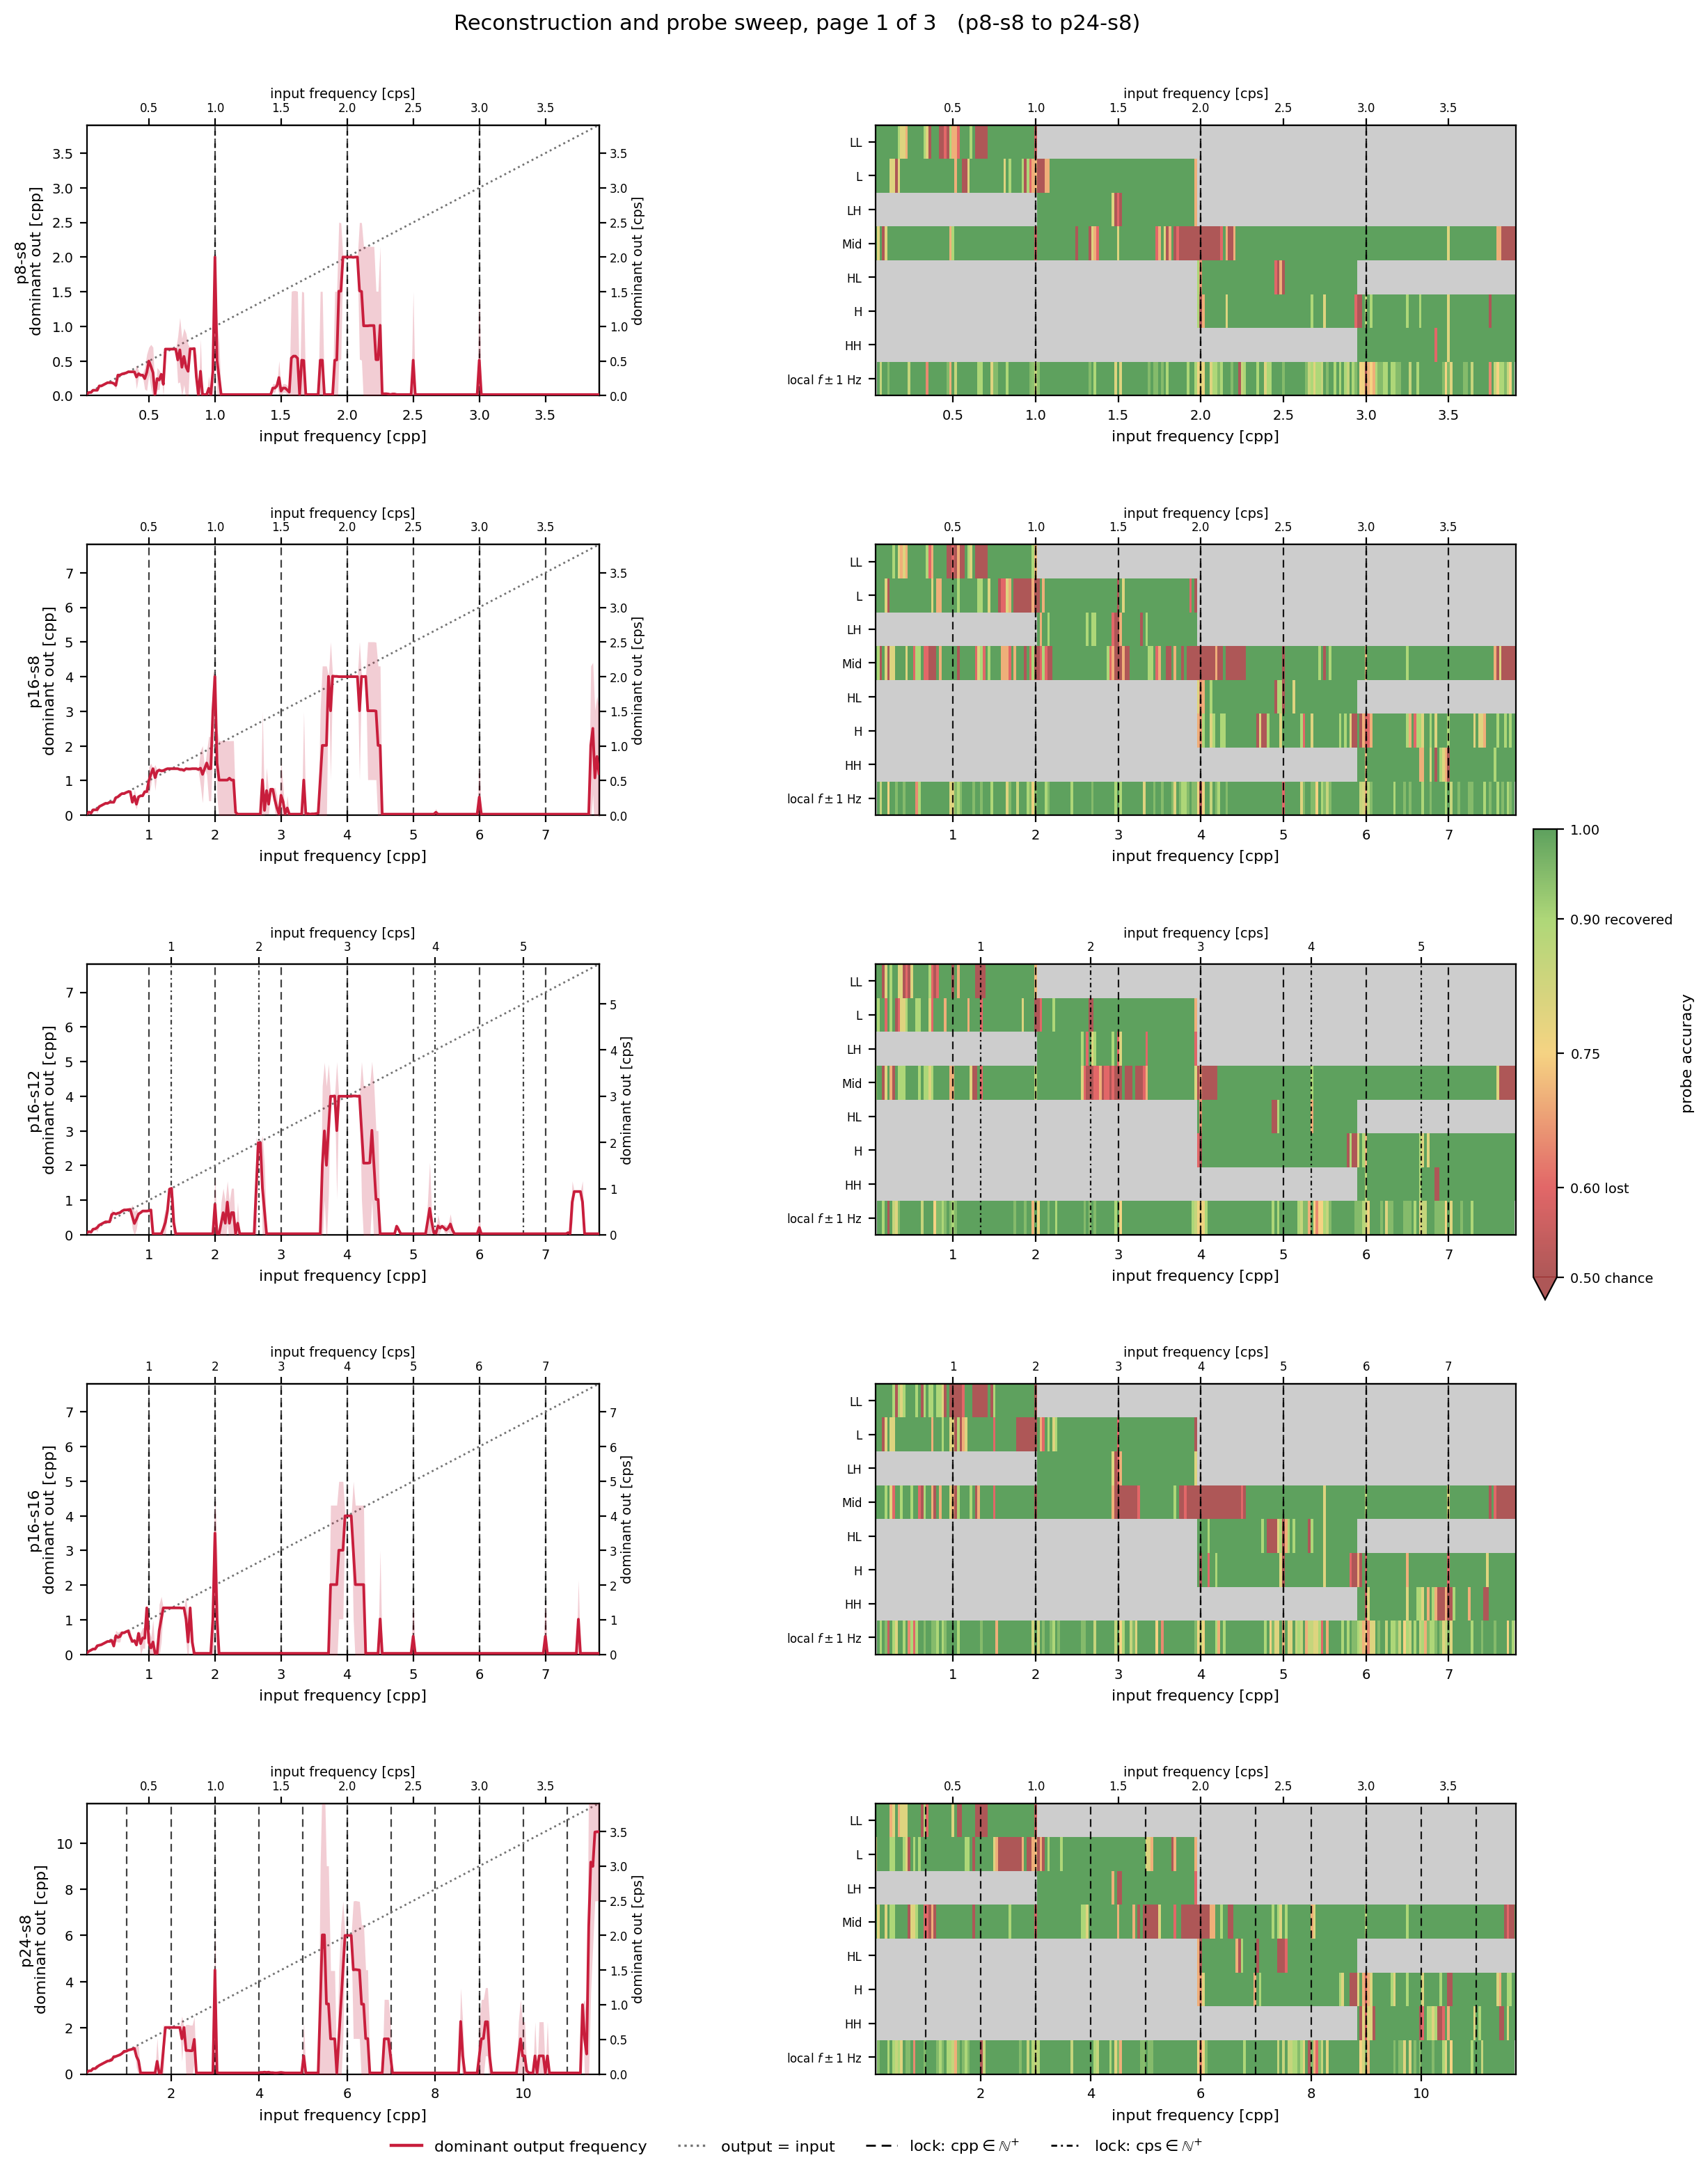
\includegraphics[width=0.8\textwidth]{figures/FIG_E1_page1.png}
    \caption{Frequency reconstruction and probe sweep, first of three: geometries p8-s8, p16-s8, p16-s12,
    p16-s16 and p24-s8. Each row is one geometry. Left, the dominant frequency of the generated
    window against the frequency supplied as context, averaged over up to four starting phases, drawn as
    the solid red curve; both axes are in cycles per patch (bottom and left) and cycles per stride
    (top and right) of that geometry. The pale red band around it is $\pm1$ standard deviation of
    that dominant frequency across the four phases: a wide band at a swept frequency means the
    frequency the model returns depends on where in its cycle the tone began, and a band that
    collapses to the curve means the reading is phase-independent there. The dotted diagonal marks
    a tone rebuilt correctly. Right, the accuracy of a linear probe on the internal state at each
    swept frequency, one strip per task, with the local $f\pm1$\,Hz task last. Dashed and dash-dotted
    verticals are that geometry's patch- and stride-branch candidates
    ($\mathrm{cpp},\mathrm{cps}\in\mathbb N^{+}$, respectively). This figure carries
    the two contiguous baselines p8-s8 and p16-s16, the geometries p16-s8 and p24-s8 that share
    $S=8$ with p8-s8, and p16-s12.}%
    \label{fig:sweepA}
\end{figure*}

\begin{figure*}[!p]
    \centering
    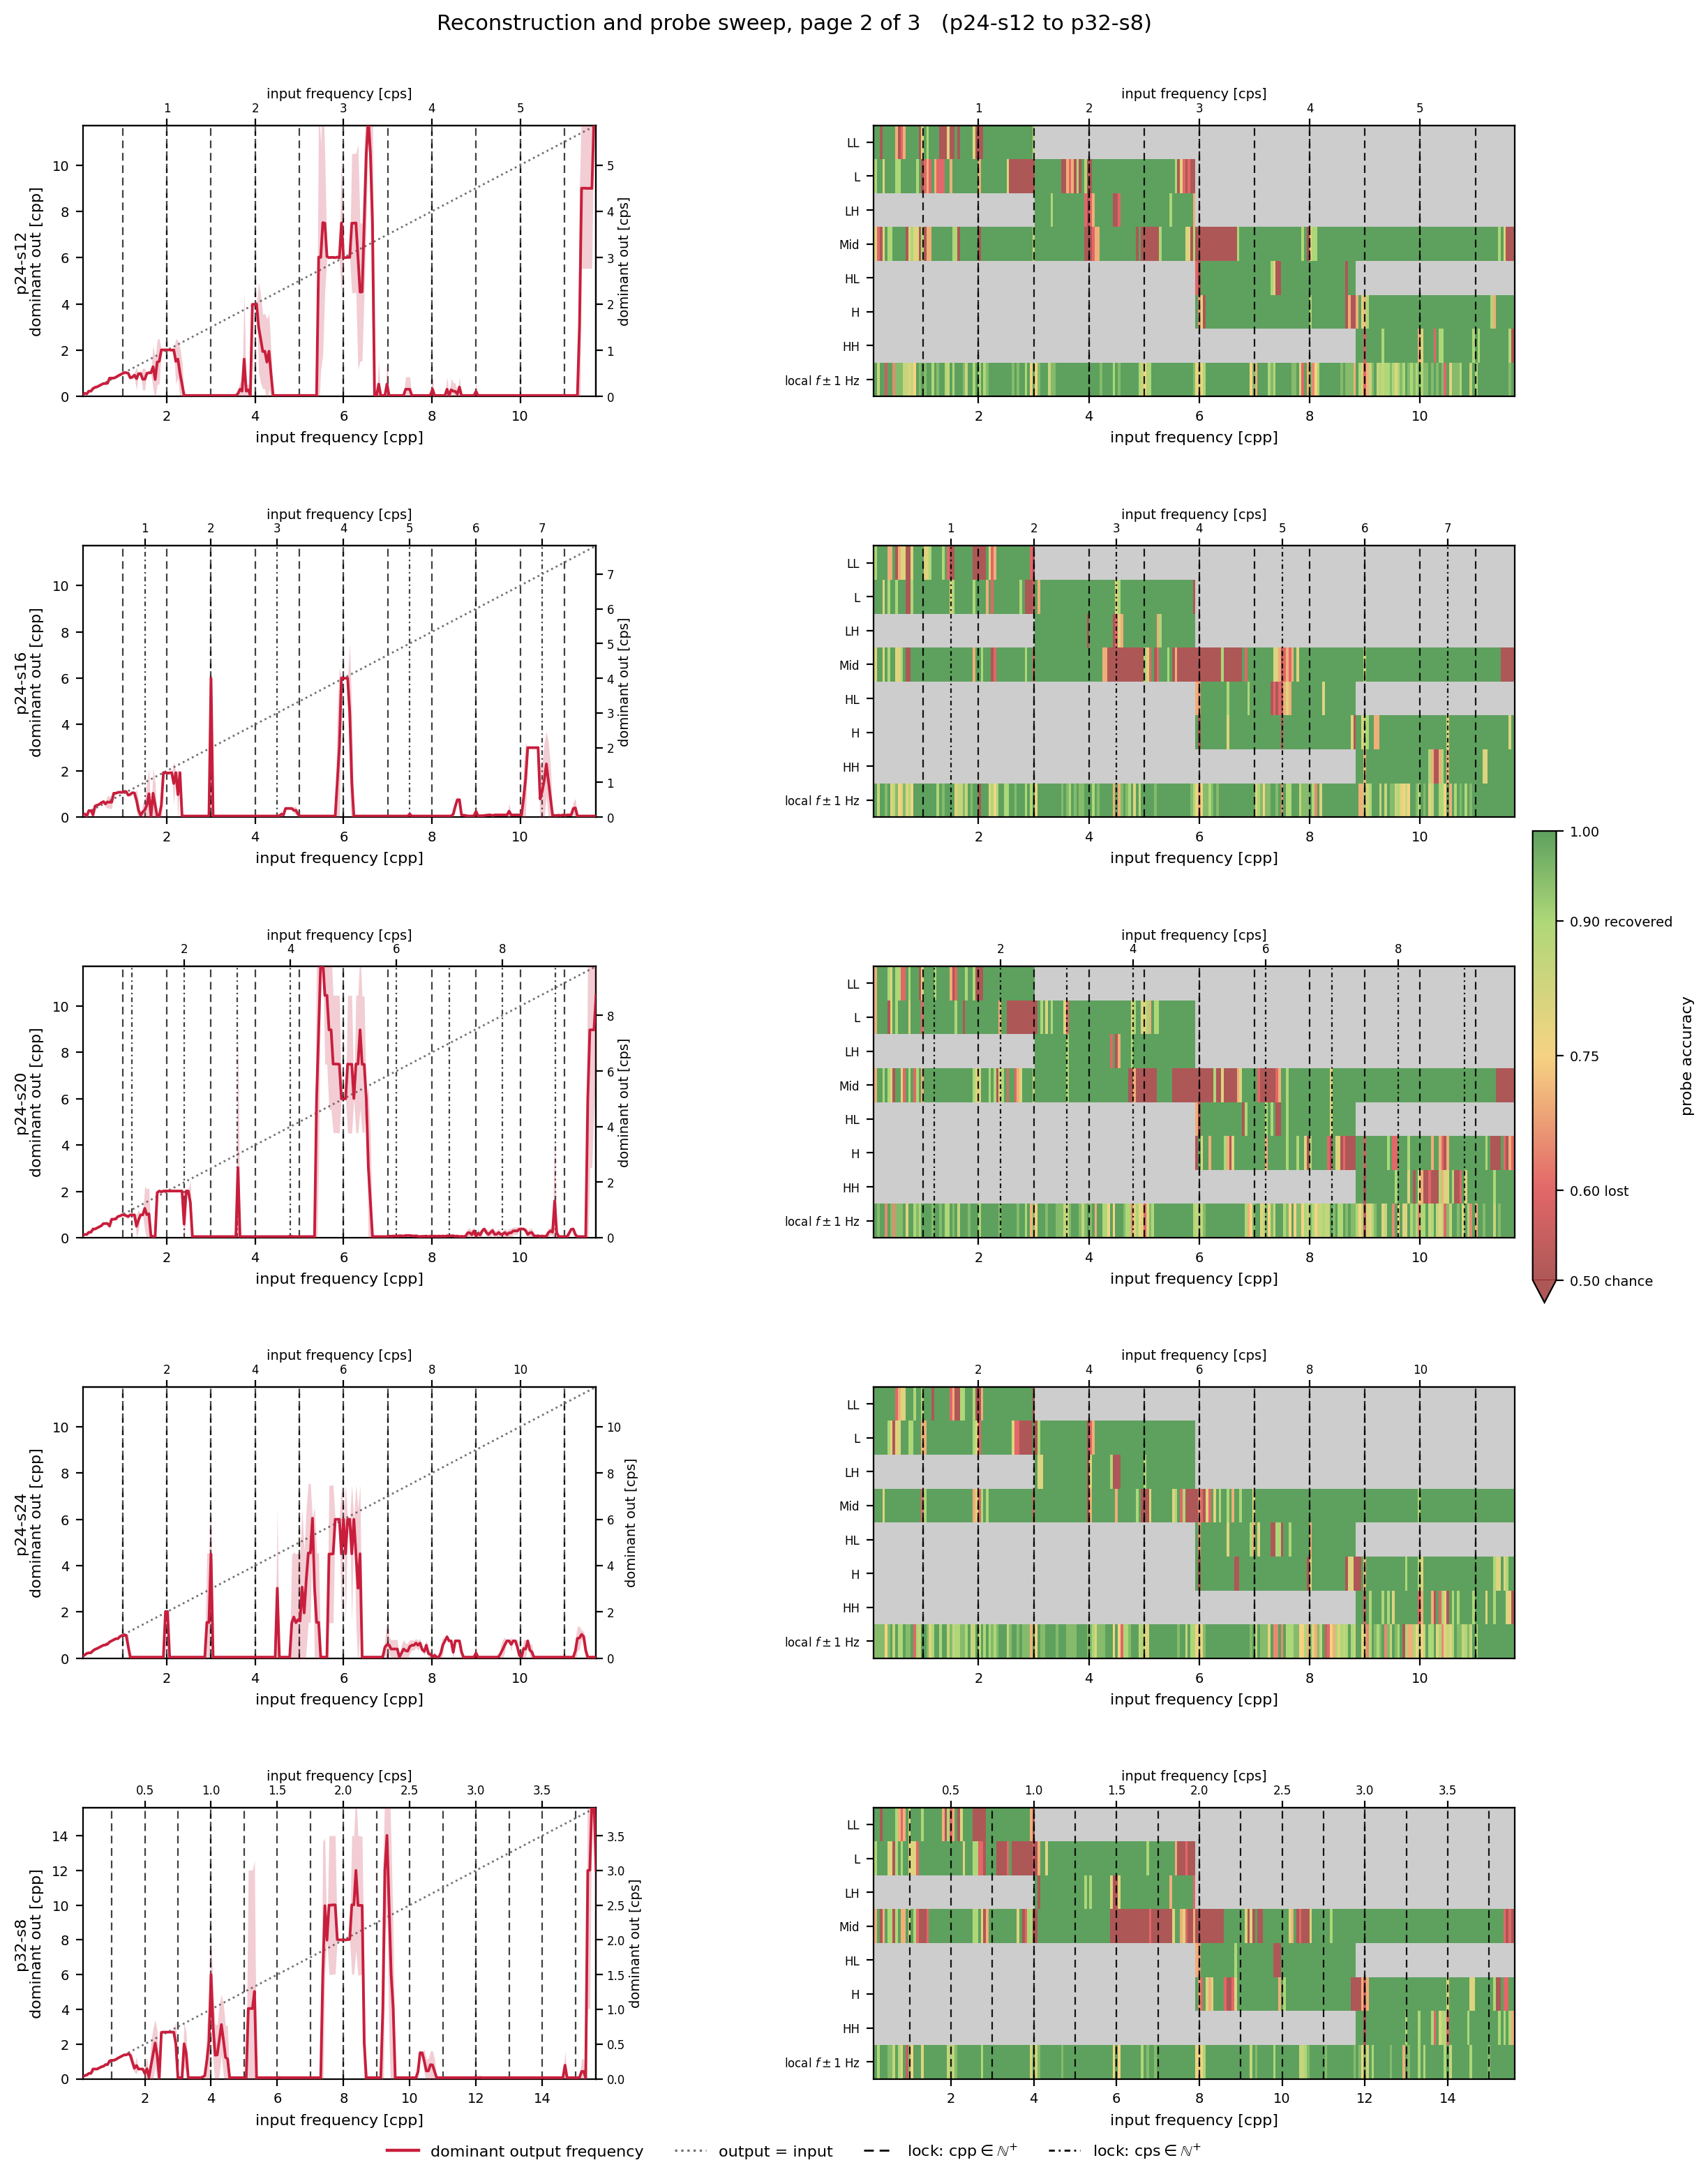
\includegraphics[width=0.85\textwidth]{figures/FIG_E1_page2.png}
    \caption{Frequency reconstruction and probe sweep, second of three: geometries p24-s12, p24-s16, p24-s20, p24-s24 and p32-s8, read as \autoref{fig:sweepA}. The first four hold the patch size at $P=24$ and shorten the stride
    from $24$ to $12$, so the stride comb $c f_s/S$ moves across the band while the patch comb
    $k f_s/P$ stays where it is: this is the series on which the two branches of
    $\mathcal F_{\mathrm{lock}}$ can be told apart by eye, and p24-s16 and p24-s20 are among the
    six runs with $S \nmid P$ on which the branch estimates rest.}%
    \label{fig:sweepB}
\end{figure*}

\begin{figure*}[!p]
    \centering
    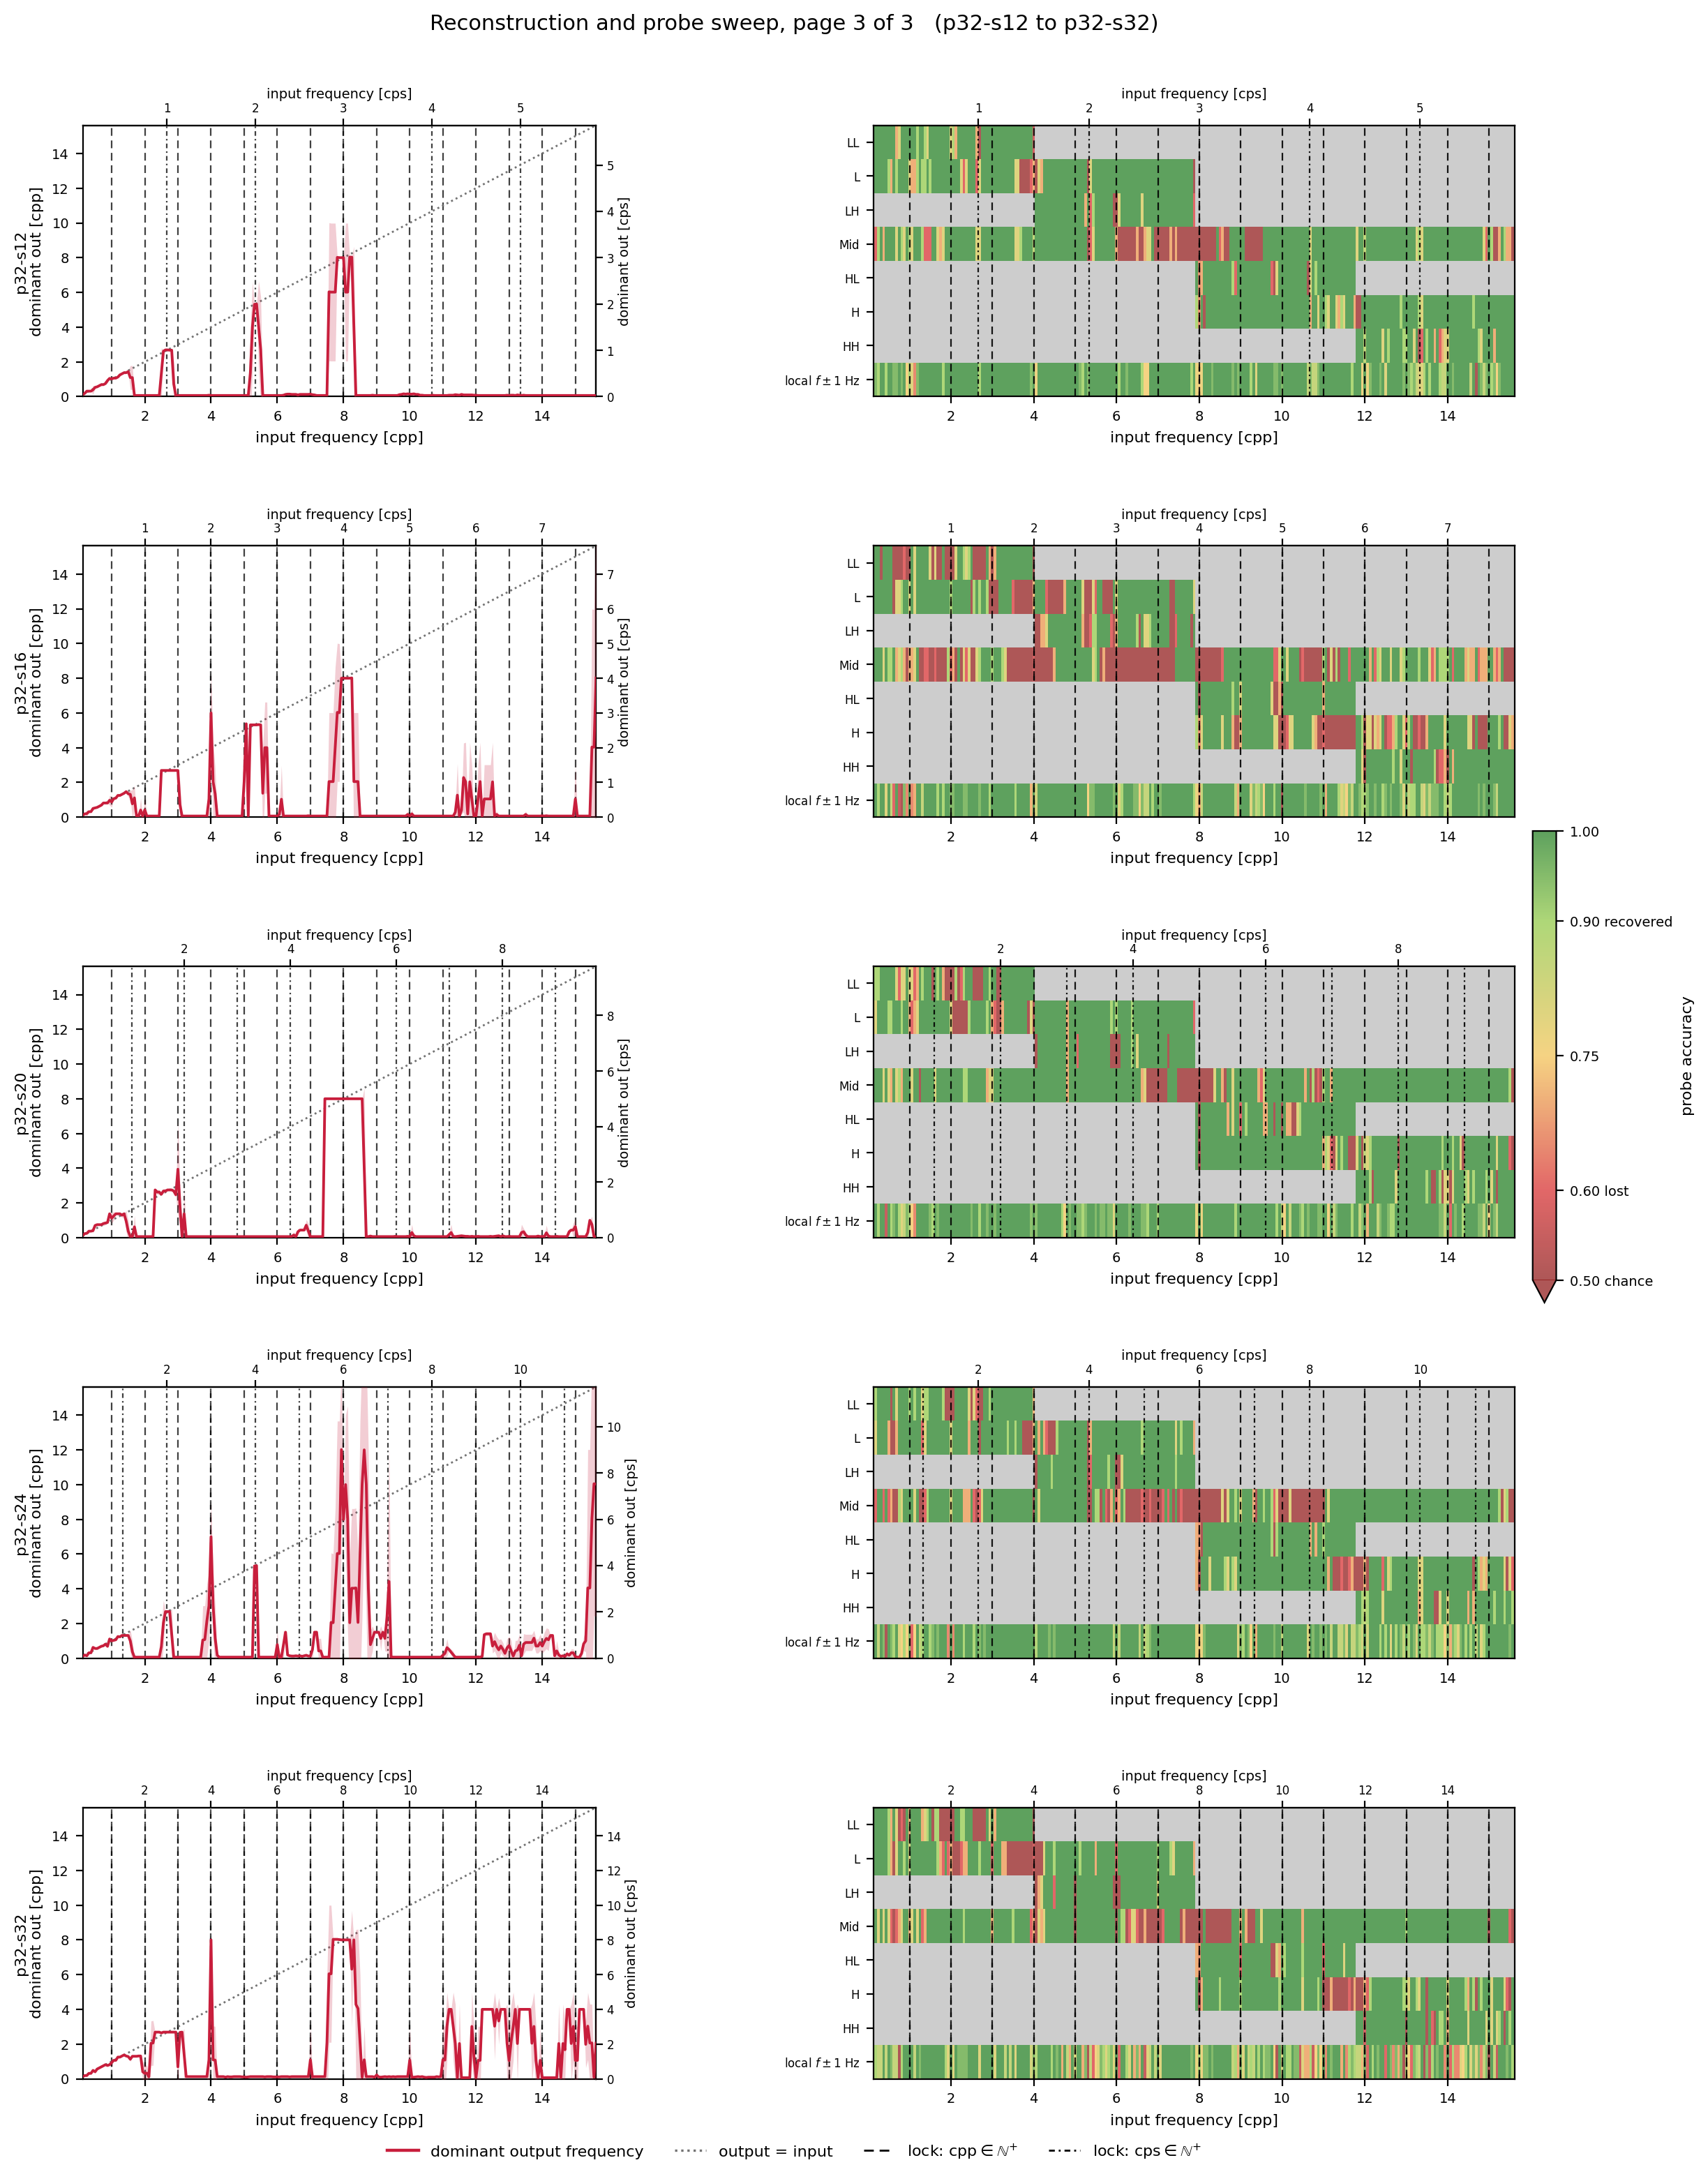
\includegraphics[width=0.85\textwidth]{figures/FIG_E1_page3.png}
    \caption{Frequency reconstruction and probe sweep, third of three: geometries p32-s12, p32-s16, p32-s20, p32-s24 and p32-s32, read as \autoref{fig:sweepA}. The patch size is held at $P=32$, the widest of the design, so the
    patch comb is the densest and the overlap ratio runs from $0.63$ down to $0$ within this one figure.
    Read against \autoref{fig:sweepB} at equal stride, the difference between the two is a difference of
    patch size alone, which is the comparison the patch-size covariate of Model~A
    is fitted to.}%
    \label{fig:sweepC}
\end{figure*}

\subsection{What is shown for each geometry}

Figures~\ref{fig:sweepA},~\ref{fig:sweepB} and~\ref{fig:sweepC} divide the design by patch size. The first carries the two smallest patches and the first $P=24$ run, where the combs are coarsest; the second completes the $P=24$ series and opens the $P=32$ block, the range over which stride varies at fixed patch size; the third holds the other five $P=32$ geometries, where the patch comb is densest, ending on $P=S=32$, where the two branches coincide.

On the left, a point on the dotted diagonal is a tone rebuilt at the frequency it was given. A flat segment means that distinct inputs return dominant frequencies in the same bin, a loss of distinguishability rather than of amplitude,\footnote{Deliverable~2 described a flat segment as distinct inputs collapsing onto one output. The reading is narrowed, following the review of Deliverable~2, because two rollouts can share their dominant bin while differing in amplitude or phase, so a flat segment shows only that the dominant frequency no longer tells the inputs apart.} and a jump is a tone the model produces that was never supplied. The shaded band is one standard deviation over the starting phases. On the right, each cell is one swept frequency coloured by probe accuracy on a continuous scale, green at or above $0.9$, yellow near $0.75$ and red below $0.6$, close to chance; grey marks a frequency no task covers. Every axis is in cycles per patch and cycles per stride of the geometry drawn, so a candidate site falls on an integer of one of the two scales. The dashed and dash-dotted verticals are the candidate sites $\mathcal F_{\mathrm{lock}}$ of the patch and stride branches, computed from $(f_s,P,S)$ and not fitted. A frequency off the diagonal on the left but green on the right was lost between the representation and the output, not at the tokenisation, while a red cell means the internal state itself no longer separates that frequency from its neighbour.

\subsection{What the figures show}

The reconstruction follows the diagonal only up to roughly one cycle per patch, and above it the output is mostly a slow component unrelated to the input: the dominant output lies within $2$\,Hz of the input for only a small minority of the swept tones in every geometry. The exceptions are tied to particular frequencies rather than scattered. Each flat segment returns a run of neighbouring inputs at one frequency, often a site of either branch. Among those sites is $f_s/4$, which lies at $2$, $4$, $6$ and $8$\,cpp for $P=8$, $16$, $24$ and $32$ and is the only frequency of the band that is a site of both branches in every geometry, because $P$ and $S$ are all multiples of four; a flat segment of several inputs sits at it in about half of the fifteen sweeps. Narrow spikes are more frequent at inputs lying on a site of either branch than at other inputs: there the output leaves the slow component and jumps, often to another site, while the neighbouring inputs do not; on p24-s20 one falls on a stride-branch site at $3$\,cps. Along a flat segment the four starting phases agree, and the phase band is widest at the steps between segments, where the output changes level.

The probe strips do not follow that pattern. The local task stays at or above $0.9$ over most of the band in every geometry, including at frequencies the reconstruction no longer places, with yellow cells that become denser towards the top of the band rather than at the sites. The band tasks are weaker, and their red cells gather at the low end of the band and beside the task boundaries of \autoref{tab:bandTasks}, most visibly in the Mid and L tasks. The boundaries of the first two levels lie next to $f_s/8$, $f_s/4$ and $3f_s/8$, sites of every geometry, and those of the third next to odd multiples of $f_s/16$, sites for $P=16$ and $P=32$. On this design, therefore, the difficulty a band task has at its own boundary cannot be told apart from an effect of the site.

These readings are descriptive, since neither is paired against controls or carries an interval. They show that the two readings disagree in a specific direction, a frequency still separated in the internal state and misplaced in the output, and that on the output the sites act as attractors rather than as holes. That observation gives the study its direction, and the Bayesian hypotheses reported in \autoref{sec:bayesResults} test it.

\subsection{Probing by stage}\label{sec:appSweepMDL}

The probe strips above read the internal state at one point only, the output quantile head, and score it by accuracy. This subsection repeats the reading at every stage of the network and scores it by description length, then compares, stage by stage, a tone on a candidate site with a tone beside it, as the recovery count of \autoref{sec:appDecomp} does on the forecast.\footnote{The probing by stage is implemented in the notebooks \href{https://github.com/FedericoSabbadini/patchAliasing/blob/main/notebooks/signal_analysis/probing_pure_tones.ipynb}{\texttt{probing\_pure\_tones.ipynb}} and \href{https://github.com/FedericoSabbadini/patchAliasing/blob/main/notebooks/signal_analysis/probing_complex_signals.ipynb}{\texttt{probing\_complex\_signals.ipynb}}.} It covers the fifteen geometries of \autoref{tab:hfModels} and the published checkpoint. Like the sweep, it is descriptive and decides no claim.

\paragraph{How the readings are produced.}

The signals are those of the sweep: pure sinusoids from $2$ to $250$\,Hz in one-hertz steps at $f_s=512$\,Hz, each at ten phases spread evenly over one cycle, so that a geometry receives $249\times10=2{,}490$ contexts, cut with the context rule of this appendix (\autoref{tab:sweepContext}). Each context passes through the network once and the state is read at ten points: the \texttt{[REG]} vector after each of the four encoder blocks, the single decoder token after each of the four decoder blocks, the input of the output projection, and its output, the quantile head.

The first reading scores the seven band tasks of \autoref{tab:bandTasks} by prequential description length\autocite{voitaInformationTheoreticProbingMinimum2020}. The contexts of a task are split into five class-stratified blocks that keep all phases of a frequency together, so that no frequency is seen in both fitting and coding. The first block is coded at one bit per label; each later block is coded by a probe, the same as in the sweep (standardisation, twenty principal components, logistic regression), fitted on the preceding blocks only. The result is the space saving $\mathrm{SV}=1-L/n$, with $L$ the code length in bits and $n$ the number of labels: positive when the state lets the labels be coded in fewer bits than one each, zero or negative when it does not. Because the first block is always paid in full, $\mathrm{SV}$ cannot exceed a ceiling between $0.77$ and $0.80$ according to the task. Two controls accompany every value. The first repeats the procedure on permuted labels. The second repeats it on a network of the same architecture with untrained weights, which reads the same contexts: what that network already exposes comes from the tokenisation and the architecture, and only the gap between the two can be attributed to training.

The second reading follows the lock and control trials of the recovery count, taken inside the network instead of on the forecast. For every candidate site of a geometry, at its exact value, a tone is placed on the site and two more beside it, one below and one above at the same offset, each more than $2$\,Hz from every candidate of that geometry. Every tone is presented at the ten phases. A tone counts as located at a stage when the three band probes on its path, the Mid task, then L or H, then one of LL, LH, HL and HH, all return its label, which places it in an eighth of the band. Those probes are fitted on the sweep without the frequencies within $1$\,Hz of the site or of its controls, so a located tone was never seen in fitting. All trials remain in each denominator. Since the task boundaries lie beside several candidate sites, the count is repeated on the pairs whose tones all lie at least $4$\,Hz from the boundaries on their path.

The same two readings are taken on complex backgrounds. The hundred Light TSMixup and the hundred KernelSynth backgrounds of \autoref{sec:appDecomp} each receive the full sweep, the tone having an amplitude of one and a half times the background standard deviation, so that each background yields its own space saving for every geometry, stage and task. Each background also keeps the site and the control it has in the recovery count, read here at ten phases by probes fitted on the sweep of that same background.

\paragraph{What is shown for each geometry.}

\autoref{fig:probingSV} draws the first reading for the reference geometry: one group of seven bars per stage, from the first encoder block at the top to the output quantile head at the bottom, one bar per band task. A bar to the right of zero is a task whose labels the stage compresses. The two values printed beside each bar are the controls, permuted labels first and untrained network second. \autoref{tab:probingStages} condenses the same reading for all geometries into the median space saving over the seven tasks at each stage, with the untrained network in its lower panel.

\autoref{tab:probingLockControl} reports the second reading: for each geometry and stage, the percentage of contexts located with the tone on a candidate site and with the tone beside it. Equal values mean that the stage places a tone as well on a site as off it, and a lower first value that the band of a tone is harder to read on a site. \autoref{tab:probingLockControlBg} gives the same pair on the two families of backgrounds, and \autoref{tab:probingCompression} the space saving at the output head across backgrounds.

% TODO(probing): replace the placeholder with the figure exported by probing_pure_tones.ipynb
%   (notebooks/signal_analysis/results/probing/fig_probing_sv_p16_s16.pdf, copy to figures/).
\begin{figure*}[!p]
    \centering
    % 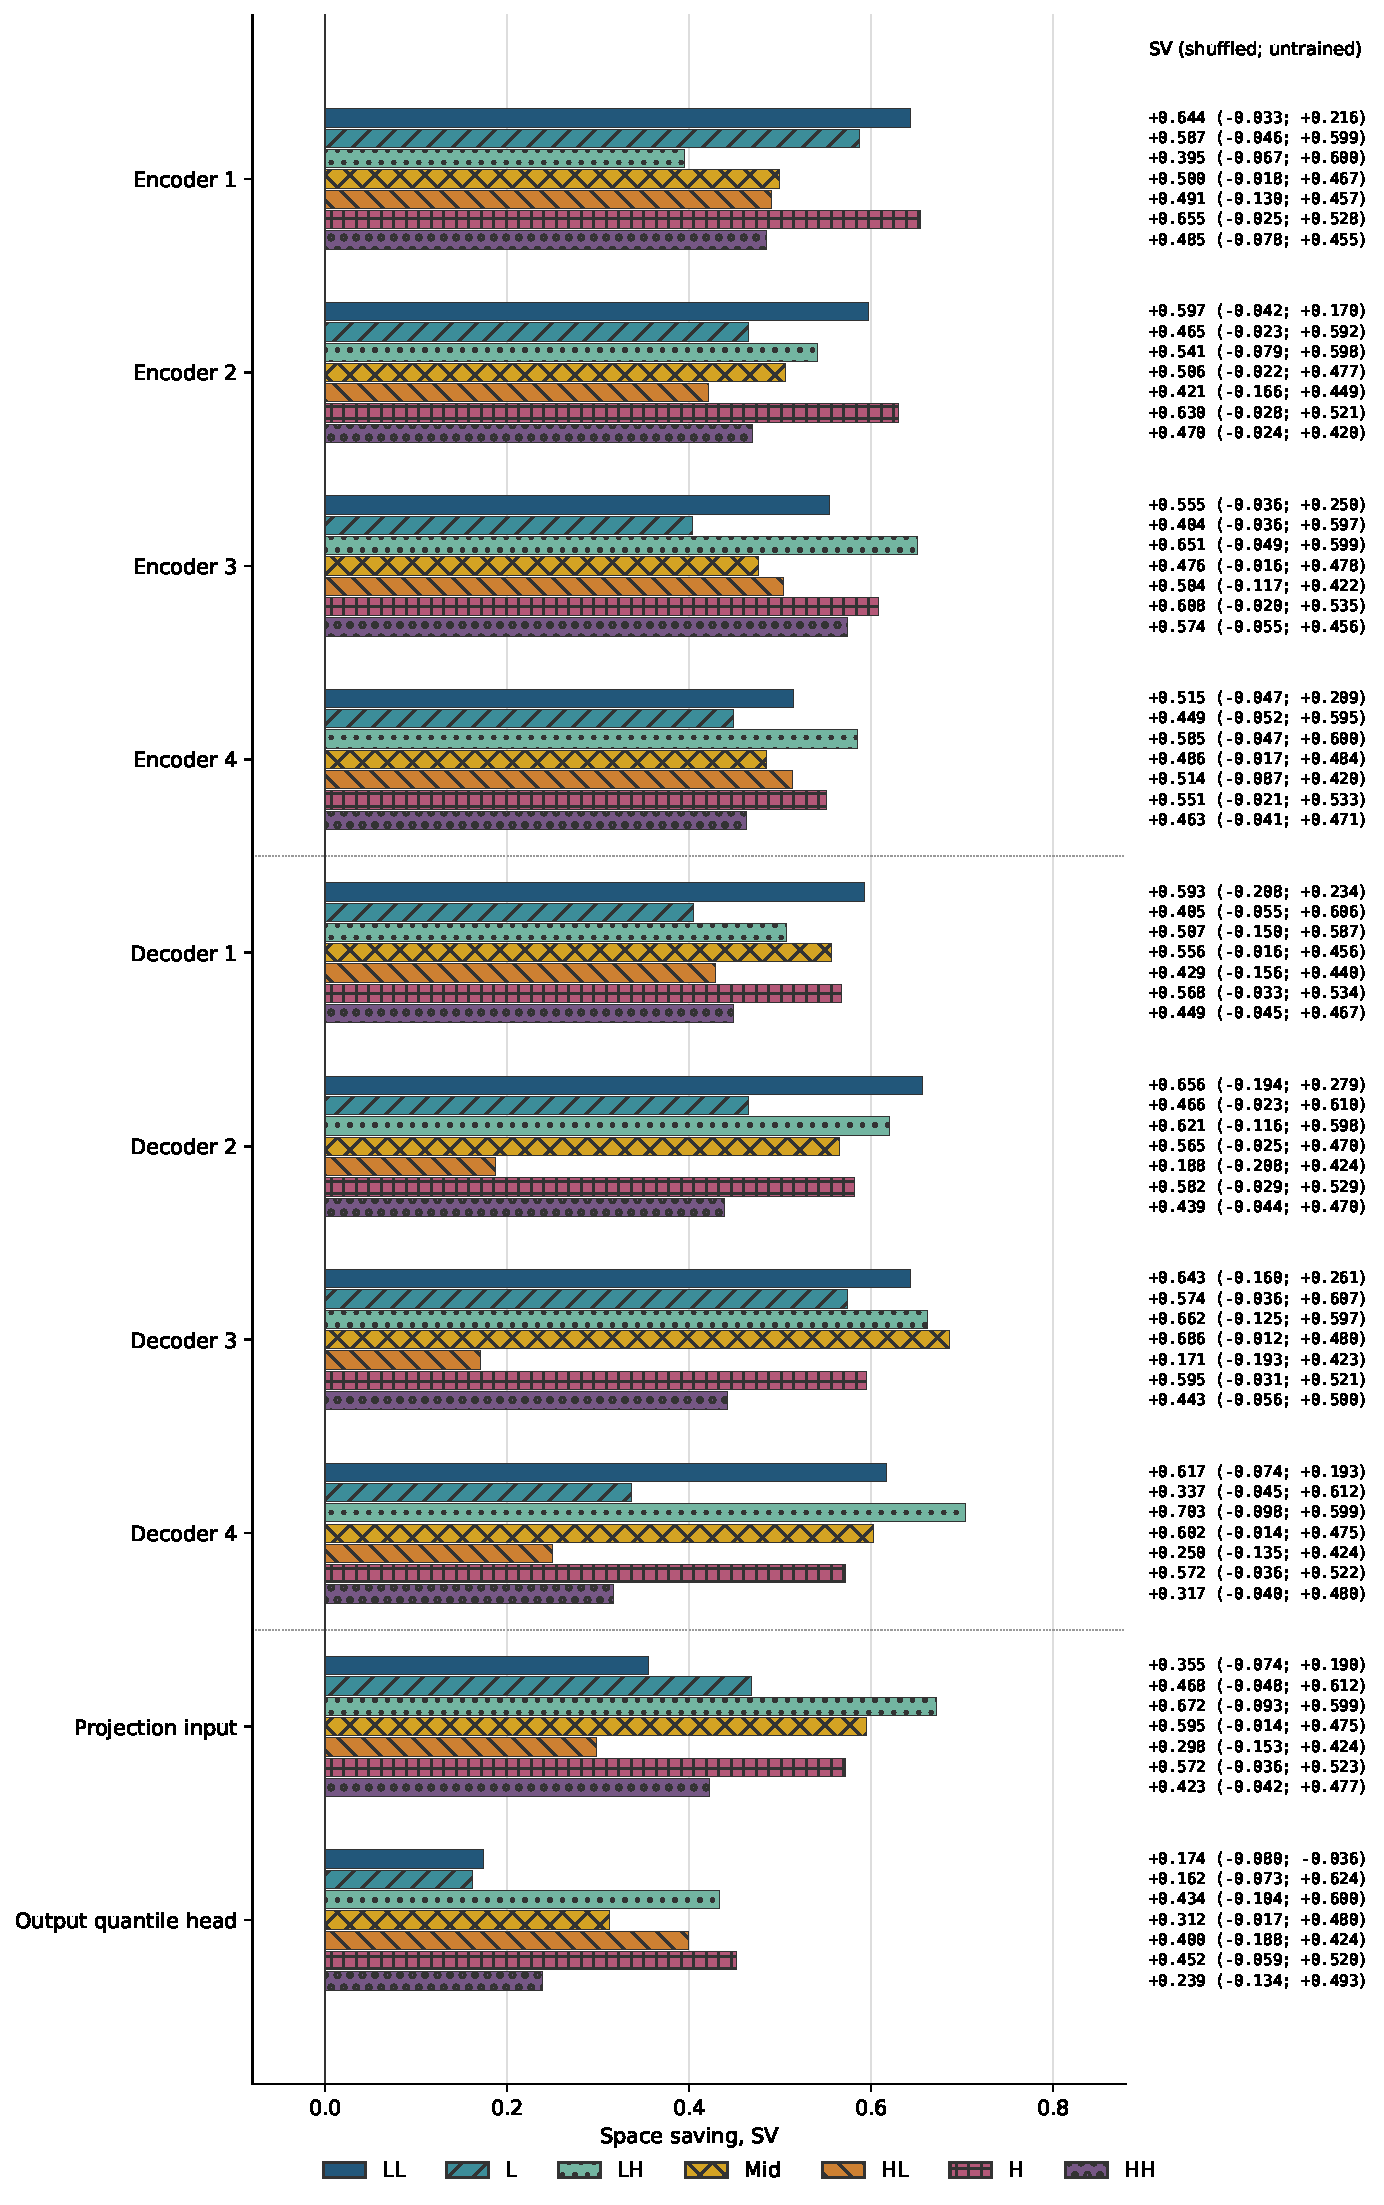
\includegraphics[width=0.75\textwidth]{figures/fig_probing_sv_p16_s16.pdf}
    \fbox{\parbox{0.75\textwidth}{\centering\vspace{3em}\textbf{TODO: figure of the pure-tone probing run}\vspace{3em}}}
    \caption{Space saving of the seven band tasks at the ten probe points, reference geometry $P=S=16$. Bars give $\mathrm{SV}=1-L/n$ under the five-block prequential code; values in parentheses are the shuffled-label and untrained-network controls. The first block is coded uniformly, which caps $\mathrm{SV}$ near $0.8$.}%
    \label{fig:probingSV}
\end{figure*}

% TODO(probing): replace each placeholder table below with the generated file, which carries the
%   same caption and label:
%   \begin{table*}[!tbp]
    \centering
    \color{red}\captionsetup{font+=probingred} % probing added after the notebook run: drop this line for the final version
    \small
    \setlength{\tabcolsep}{3.5pt}
    \begin{tabular}{@{}ccrrrrrrrrrr@{}}
        \toprule
        \multicolumn{12}{c}{\textbf{Trained network}} \\
        \midrule
        \textbf{$P$} & \textbf{$S$} & \textbf{E1} & \textbf{E2} & \textbf{E3} & \textbf{E4} & \textbf{D1} & \textbf{D2} & \textbf{D3} & \textbf{D4} & \textbf{In} & \textbf{Head} \\
        \midrule
        $16$ & $16^{\dagger}$ & $0.75$ & $0.74$ & $0.75$ & $0.75$ & $0.74$ & $0.76$ & $0.70$ & $0.70$ & $0.70$ & $0.37$ \\
        \midrule
        \addlinespace[2pt]
        $8$ & $8$ & $0.70$ & $0.70$ & $0.70$ & $0.68$ & $0.67$ & $0.70$ & $0.68$ & $0.63$ & $0.65$ & $0.45$ \\
        \addlinespace[2pt]
        $16$ & $8$ & $0.64$ & $0.61$ & $0.68$ & $0.67$ & $0.54$ & $0.57$ & $0.56$ & $0.58$ & $0.53$ & $0.26$ \\
        $16$ & $12$ & $0.60$ & $0.63$ & $0.54$ & $0.57$ & $0.55$ & $0.65$ & $0.64$ & $0.60$ & $0.59$ & $0.37$ \\
        $16$ & $16$ & $0.50$ & $0.51$ & $0.55$ & $0.51$ & $0.51$ & $0.56$ & $0.60$ & $0.57$ & $0.47$ & $0.31$ \\
        \addlinespace[2pt]
        $24$ & $8$ & $0.59$ & $0.61$ & $0.56$ & $0.51$ & $0.49$ & $0.54$ & $0.49$ & $0.52$ & $0.52$ & $0.23$ \\
        $24$ & $12$ & $0.54$ & $0.51$ & $0.51$ & $0.51$ & $0.58$ & $0.63$ & $0.65$ & $0.62$ & $0.60$ & $0.28$ \\
        $24$ & $16$ & $0.37$ & $0.35$ & $0.39$ & $0.40$ & $0.55$ & $0.61$ & $0.65$ & $0.58$ & $0.54$ & $0.33$ \\
        $24$ & $20$ & $0.54$ & $0.49$ & $0.51$ & $0.54$ & $0.59$ & $0.52$ & $0.62$ & $0.58$ & $0.56$ & $0.28$ \\
        $24$ & $24$ & $0.43$ & $0.42$ & $0.41$ & $0.42$ & $0.52$ & $0.42$ & $0.41$ & $0.45$ & $0.46$ & $0.38$ \\
        \addlinespace[2pt]
        $32$ & $8$ & $0.46$ & $0.42$ & $0.43$ & $0.49$ & $0.32$ & $0.38$ & $0.42$ & $0.47$ & $0.51$ & $0.14$ \\
        $32$ & $12$ & $0.39$ & $0.43$ & $0.45$ & $0.47$ & $0.50$ & $0.52$ & $0.53$ & $0.52$ & $0.52$ & $0.30$ \\
        $32$ & $16$ & $0.21$ & $0.37$ & $0.44$ & $0.43$ & $0.49$ & $0.48$ & $0.53$ & $0.45$ & $0.40$ & $-0.04$ \\
        $32$ & $20$ & $0.44$ & $0.46$ & $0.49$ & $0.47$ & $0.48$ & $0.36$ & $0.43$ & $0.43$ & $0.41$ & $0.25$ \\
        $32$ & $24$ & $0.53$ & $0.57$ & $0.55$ & $0.46$ & $0.52$ & $0.54$ & $0.50$ & $0.49$ & $0.47$ & $0.22$ \\
        $32$ & $32$ & $0.28$ & $0.42$ & $0.31$ & $0.33$ & $0.37$ & $0.35$ & $0.35$ & $0.38$ & $0.35$ & $0.27$ \\
        \midrule
        \multicolumn{12}{c}{\textbf{Untrained network}} \\
        \midrule
        \textbf{$P$} & \textbf{$S$} & \textbf{E1} & \textbf{E2} & \textbf{E3} & \textbf{E4} & \textbf{D1} & \textbf{D2} & \textbf{D3} & \textbf{D4} & \textbf{In} & \textbf{Head} \\
        \midrule
        $16$ & $16^{\dagger}$ & $0.47$ & $0.48$ & $0.48$ & $0.48$ & $0.47$ & $0.47$ & $0.50$ & $0.48$ & $0.48$ & $0.49$ \\
        \midrule
        \addlinespace[2pt]
        $8$ & $8$ & $0.64$ & $0.64$ & $0.64$ & $0.62$ & $0.61$ & $0.64$ & $0.64$ & $0.64$ & $0.64$ & $0.65$ \\
        \addlinespace[2pt]
        $16$ & $8$ & $0.65$ & $0.66$ & $0.65$ & $0.65$ & $0.61$ & $0.64$ & $0.65$ & $0.63$ & $0.63$ & $0.65$ \\
        $16$ & $12$ & $0.58$ & $0.57$ & $0.58$ & $0.60$ & $0.57$ & $0.58$ & $0.59$ & $0.57$ & $0.57$ & $0.59$ \\
        $16$ & $16$ & $0.47$ & $0.48$ & $0.48$ & $0.48$ & $0.47$ & $0.47$ & $0.50$ & $0.48$ & $0.48$ & $0.49$ \\
        \addlinespace[2pt]
        $24$ & $8$ & $0.62$ & $0.65$ & $0.65$ & $0.69$ & $0.62$ & $0.67$ & $0.69$ & $0.65$ & $0.65$ & $0.65$ \\
        $24$ & $12$ & $0.53$ & $0.61$ & $0.59$ & $0.54$ & $0.54$ & $0.60$ & $0.55$ & $0.51$ & $0.52$ & $0.59$ \\
        $24$ & $16$ & $0.48$ & $0.50$ & $0.52$ & $0.53$ & $0.53$ & $0.52$ & $0.54$ & $0.53$ & $0.53$ & $0.56$ \\
        $24$ & $20$ & $0.59$ & $0.56$ & $0.61$ & $0.58$ & $0.56$ & $0.59$ & $0.57$ & $0.57$ & $0.57$ & $0.63$ \\
        $24$ & $24$ & $0.49$ & $0.51$ & $0.51$ & $0.53$ & $0.51$ & $0.48$ & $0.48$ & $0.48$ & $0.48$ & $0.52$ \\
        \addlinespace[2pt]
        $32$ & $8$ & $0.56$ & $0.57$ & $0.59$ & $0.59$ & $0.58$ & $0.58$ & $0.58$ & $0.58$ & $0.58$ & $0.59$ \\
        $32$ & $12$ & $0.43$ & $0.54$ & $0.54$ & $0.48$ & $0.55$ & $0.48$ & $0.52$ & $0.54$ & $0.54$ & $0.54$ \\
        $32$ & $16$ & $0.40$ & $0.45$ & $0.46$ & $0.44$ & $0.46$ & $0.40$ & $0.43$ & $0.42$ & $0.39$ & $0.40$ \\
        $32$ & $20$ & $0.46$ & $0.47$ & $0.45$ & $0.46$ & $0.43$ & $0.42$ & $0.44$ & $0.45$ & $0.45$ & $0.46$ \\
        $32$ & $24$ & $0.43$ & $0.45$ & $0.46$ & $0.43$ & $0.45$ & $0.47$ & $0.48$ & $0.48$ & $0.48$ & $0.52$ \\
        $32$ & $32$ & $0.20$ & $0.21$ & $0.18$ & $0.19$ & $0.14$ & $0.21$ & $0.18$ & $0.16$ & $0.15$ & $0.20$ \\
        \bottomrule
    \end{tabular}
    \caption{Median space saving over the seven band tasks at each probe point, pure tones. E1--E4 and D1--D4 are the encoder and decoder blocks, In the input of the output projection and Head the output quantile head. The lower panel repeats the reading on the same architecture with untrained weights. $\dagger$ marks the published checkpoint.}
    \label{tab:probingStages}
\end{table*}
                  (pure tones, tab:probingStages)
%   \begin{table*}[!tbp]
    \centering
    \color{red}\captionsetup{font+=probingred} % probing added after the notebook run: drop this line for the final version
    \small
    \setlength{\tabcolsep}{3.5pt}
    \begin{tabular}{@{}cccccccccccc@{}}
        \toprule
        \textbf{$P$} & \textbf{$S$} & \textbf{E1} & \textbf{E2} & \textbf{E3} & \textbf{E4} & \textbf{D1} & \textbf{D2} & \textbf{D3} & \textbf{D4} & \textbf{In} & \textbf{Head} \\
        \midrule
        $16$ & $16^{\dagger}$ & $51/100$ & $49/100$ & $47/100$ & $44/100$ & $50/100$ & $46/96$ & $59/94$ & $64/93$ & $63/96$ & $40/78$ \\
        \midrule
        \addlinespace[2pt]
        $8$ & $8$ & $40/82$ & $23/88$ & $33/98$ & $43/100$ & $37/95$ & $37/97$ & $43/97$ & $47/95$ & $37/93$ & $33/85$ \\
        \addlinespace[2pt]
        $16$ & $8$ & $39/98$ & $41/94$ & $43/88$ & $36/90$ & $29/85$ & $31/84$ & $17/86$ & $27/90$ & $14/84$ & $26/63$ \\
        $16$ & $12$ & $45/81$ & $40/89$ & $41/83$ & $48/87$ & $45/99$ & $35/100$ & $39/100$ & $38/100$ & $37/95$ & $30/81$ \\
        $16$ & $16$ & $27/82$ & $34/81$ & $30/84$ & $36/76$ & $21/96$ & $29/99$ & $31/97$ & $33/89$ & $29/89$ & $20/65$ \\
        \addlinespace[2pt]
        $24$ & $8$ & $73/88$ & $76/87$ & $66/89$ & $68/80$ & $63/79$ & $57/87$ & $55/83$ & $50/87$ & $58/84$ & $42/73$ \\
        $24$ & $12$ & $45/75$ & $44/77$ & $44/74$ & $42/70$ & $44/92$ & $42/88$ & $47/91$ & $45/93$ & $47/88$ & $25/70$ \\
        $24$ & $16$ & $39/73$ & $37/73$ & $43/74$ & $40/74$ & $57/92$ & $57/94$ & $57/97$ & $57/96$ & $48/93$ & $48/75$ \\
        $24$ & $20$ & $64/81$ & $56/81$ & $50/73$ & $50/73$ & $58/91$ & $66/94$ & $65/87$ & $67/90$ & $61/83$ & $38/65$ \\
        $24$ & $24$ & $42/82$ & $45/86$ & $44/85$ & $46/85$ & $24/95$ & $29/93$ & $34/94$ & $37/95$ & $35/92$ & $17/85$ \\
        \addlinespace[2pt]
        $32$ & $8$ & $58/66$ & $60/68$ & $61/69$ & $63/71$ & $59/75$ & $60/83$ & $59/83$ & $64/82$ & $59/81$ & $53/54$ \\
        $32$ & $12$ & $48/53$ & $50/57$ & $54/58$ & $55/57$ & $66/85$ & $65/87$ & $62/83$ & $58/86$ & $65/86$ & $54/69$ \\
        $32$ & $16$ & $37/49$ & $36/60$ & $38/68$ & $38/70$ & $39/95$ & $39/80$ & $40/71$ & $41/73$ & $41/76$ & $23/35$ \\
        $32$ & $20$ & $43/75$ & $42/76$ & $48/79$ & $48/76$ & $60/87$ & $60/92$ & $58/92$ & $60/92$ & $58/92$ & $45/75$ \\
        $32$ & $24$ & $46/78$ & $47/83$ & $51/82$ & $53/83$ & $56/92$ & $54/91$ & $58/88$ & $55/91$ & $58/92$ & $36/64$ \\
        $32$ & $32$ & $39/64$ & $36/70$ & $41/69$ & $44/68$ & $43/85$ & $40/77$ & $45/74$ & $41/76$ & $42/80$ & $31/53$ \\
        \bottomrule
    \end{tabular}
    \caption{Pure tones located at each probe point, in per cent of the contexts, at the candidate sites of each geometry and at the controls beside them (lock/control). A tone is located when the three band probes on its path all return its label; the probes are fitted without the frequencies within $1$\,Hz of the tone. Columns as in \autoref{tab:probingStages}. $\dagger$ marks the published checkpoint.}
    \label{tab:probingLockControl}
\end{table*}
               (pure tones, tab:probingLockControl)
%   \begin{table*}[!tbp]
    \centering
    \color{red}\captionsetup{font+=probingred} % probing added after the notebook run: drop this line for the final version
    \small
    \setlength{\tabcolsep}{3.5pt}
    \begin{tabular}{@{}cccccccccccc@{}}
        \toprule
        \multicolumn{12}{c}{\textbf{Light TSMixup}} \\
        \midrule
        \textbf{$P$} & \textbf{$S$} & \textbf{E1} & \textbf{E2} & \textbf{E3} & \textbf{E4} & \textbf{D1} & \textbf{D2} & \textbf{D3} & \textbf{D4} & \textbf{In} & \textbf{Head} \\
        \midrule
        $16$ & $16^{\dagger}$ & $51/97$ & $47/96$ & $49/97$ & $46/94$ & $48/95$ & $47/91$ & $50/94$ & $50/88$ & $51/90$ & $37/60$ \\
        \midrule
        \addlinespace[2pt]
        $8$ & $8$ & $39/80$ & $32/84$ & $32/88$ & $34/94$ & $17/97$ & $26/97$ & $32/98$ & $37/94$ & $30/95$ & $18/88$ \\
        \addlinespace[2pt]
        $16$ & $8$ & $40/90$ & $42/88$ & $41/87$ & $35/87$ & $35/80$ & $35/78$ & $34/82$ & $36/87$ & $29/82$ & $26/66$ \\
        $16$ & $12$ & $41/66$ & $38/70$ & $38/69$ & $39/68$ & $46/92$ & $44/94$ & $46/93$ & $47/93$ & $43/91$ & $38/72$ \\
        $16$ & $16$ & $29/68$ & $34/70$ & $30/67$ & $34/63$ & $28/90$ & $30/90$ & $33/90$ & $31/85$ & $26/82$ & $25/66$ \\
        \addlinespace[2pt]
        $24$ & $8$ & $72/74$ & $71/75$ & $66/79$ & $64/72$ & $62/79$ & $66/80$ & $63/78$ & $64/79$ & $66/77$ & $49/56$ \\
        $24$ & $12$ & $42/72$ & $41/71$ & $42/70$ & $44/71$ & $49/85$ & $48/86$ & $46/85$ & $48/85$ & $46/81$ & $35/59$ \\
        $24$ & $16$ & $36/67$ & $35/66$ & $38/68$ & $39/68$ & $52/81$ & $54/88$ & $56/88$ & $53/88$ & $52/88$ & $43/66$ \\
        $24$ & $20$ & $55/68$ & $52/68$ & $48/64$ & $48/61$ & $58/78$ & $58/83$ & $61/80$ & $56/77$ & $56/75$ & $44/58$ \\
        $24$ & $24$ & $39/65$ & $39/70$ & $39/69$ & $40/69$ & $31/76$ & $34/72$ & $35/74$ & $35/73$ & $36/73$ & $24/59$ \\
        \addlinespace[2pt]
        $32$ & $8$ & $45/56$ & $46/57$ & $47/60$ & $51/60$ & $60/72$ & $60/73$ & $62/76$ & $62/74$ & $62/74$ & $54/60$ \\
        $32$ & $12$ & $45/50$ & $47/53$ & $46/55$ & $50/60$ & $61/75$ & $63/79$ & $57/76$ & $56/73$ & $59/72$ & $44/59$ \\
        $32$ & $16$ & $34/48$ & $36/52$ & $38/56$ & $39/59$ & $47/88$ & $46/78$ & $47/74$ & $48/75$ & $45/69$ & $31/41$ \\
        $32$ & $20$ & $37/64$ & $38/64$ & $40/64$ & $41/65$ & $56/77$ & $57/82$ & $58/83$ & $60/84$ & $58/82$ & $46/61$ \\
        $32$ & $24$ & $43/61$ & $47/64$ & $45/63$ & $48/63$ & $55/84$ & $55/82$ & $53/81$ & $52/77$ & $57/81$ & $44/57$ \\
        $32$ & $32$ & $36/46$ & $41/53$ & $39/50$ & $40/48$ & $44/70$ & $45/63$ & $42/63$ & $41/62$ & $42/62$ & $31/49$ \\
        \midrule
        \multicolumn{12}{c}{\textbf{KernelSynth}} \\
        \midrule
        \textbf{$P$} & \textbf{$S$} & \textbf{E1} & \textbf{E2} & \textbf{E3} & \textbf{E4} & \textbf{D1} & \textbf{D2} & \textbf{D3} & \textbf{D4} & \textbf{In} & \textbf{Head} \\
        \midrule
        $16$ & $16^{\dagger}$ & $53/98$ & $52/99$ & $50/99$ & $45/98$ & $48/98$ & $48/96$ & $51/95$ & $55/94$ & $55/95$ & $42/71$ \\
        \midrule
        \addlinespace[2pt]
        $8$ & $8$ & $41/80$ & $37/87$ & $31/93$ & $30/94$ & $16/95$ & $24/95$ & $34/96$ & $36/92$ & $29/94$ & $19/88$ \\
        \addlinespace[2pt]
        $16$ & $8$ & $39/88$ & $38/87$ & $38/84$ & $34/82$ & $35/75$ & $33/78$ & $32/80$ & $31/84$ & $29/84$ & $24/76$ \\
        $16$ & $12$ & $41/73$ & $35/74$ & $34/75$ & $36/74$ & $40/87$ & $42/89$ & $44/89$ & $41/90$ & $40/88$ & $37/77$ \\
        $16$ & $16$ & $28/72$ & $34/76$ & $32/72$ & $31/68$ & $28/89$ & $33/87$ & $33/89$ & $32/85$ & $27/86$ & $30/72$ \\
        \addlinespace[2pt]
        $24$ & $8$ & $69/78$ & $65/76$ & $67/76$ & $62/74$ & $56/81$ & $58/81$ & $54/80$ & $54/79$ & $56/79$ & $46/65$ \\
        $24$ & $12$ & $41/69$ & $42/71$ & $41/73$ & $42/74$ & $44/82$ & $46/85$ & $45/85$ & $44/85$ & $42/82$ & $36/65$ \\
        $24$ & $16$ & $38/70$ & $39/73$ & $43/76$ & $43/75$ & $50/84$ & $57/88$ & $53/87$ & $53/86$ & $49/84$ & $44/71$ \\
        $24$ & $20$ & $54/70$ & $53/71$ & $47/63$ & $48/60$ & $56/77$ & $58/77$ & $60/76$ & $56/76$ & $56/76$ & $46/60$ \\
        $24$ & $24$ & $36/69$ & $40/72$ & $40/72$ & $40/74$ & $28/77$ & $31/75$ & $32/76$ & $33/76$ & $32/74$ & $26/64$ \\
        \addlinespace[2pt]
        $32$ & $8$ & $51/58$ & $56/60$ & $56/63$ & $60/65$ & $58/74$ & $62/74$ & $64/73$ & $64/74$ & $62/74$ & $54/65$ \\
        $32$ & $12$ & $47/53$ & $51/57$ & $54/62$ & $55/61$ & $61/80$ & $60/80$ & $56/77$ & $53/73$ & $58/73$ & $48/66$ \\
        $32$ & $16$ & $33/48$ & $35/56$ & $39/58$ & $40/62$ & $40/78$ & $44/70$ & $45/66$ & $46/67$ & $43/67$ & $34/47$ \\
        $32$ & $20$ & $44/67$ & $43/68$ & $44/67$ & $45/66$ & $56/76$ & $56/80$ & $55/80$ & $57/80$ & $57/78$ & $50/63$ \\
        $32$ & $24$ & $44/65$ & $47/69$ & $49/67$ & $51/68$ & $56/84$ & $57/84$ & $55/83$ & $52/79$ & $57/84$ & $49/65$ \\
        $32$ & $32$ & $40/51$ & $38/54$ & $35/54$ & $41/57$ & $42/66$ & $42/63$ & $41/61$ & $39/66$ & $39/66$ & $30/49$ \\
        \bottomrule
    \end{tabular}
    \caption{Added tones located at each probe point, in per cent of the contexts, when the tone sits on a candidate site and when it sits beside it (lock/control), over $100$ backgrounds per generator. Sites and controls are those of the recovery count (\autoref{tab:decomposition}), and the probes never saw the frequencies within $1$\,Hz of the tone. Columns as in \autoref{tab:probingLockControl}. $\dagger$ marks the published checkpoint.}
    \label{tab:probingLockControlBg}
\end{table*}
   (KS/TSM,     tab:probingLockControlBg)
%   \begin{table*}[!tbp]
    \centering
    \color{red}\captionsetup{font+=probingred} % probing added after the notebook run: drop this line for the final version
    \small
    \setlength{\tabcolsep}{5pt}
    \begin{tabular}{@{}ccrrrrrrr@{}}
        \toprule
        \multicolumn{9}{c}{\textbf{Light TSMixup}} \\
        \midrule
        \textbf{$P$} & \textbf{$S$} & \textbf{LL} & \textbf{L} & \textbf{LH} & \textbf{Mid} & \textbf{HL} & \textbf{H} & \textbf{HH} \\
        \midrule
        $16$ & $16^{\dagger}$ & $-0.05_{-0.16}^{0.05}$ & $-0.00_{-0.04}^{0.08}$ & $0.04_{-0.07}^{0.21}$ & $0.31_{0.21}^{0.43}$ & $0.35_{0.24}^{0.43}$ & $0.49_{0.42}^{0.57}$ & $0.33_{0.24}^{0.40}$ \\
        \midrule
        \addlinespace[2pt]
        $8$ & $8$ & $0.24_{0.16}^{0.29}$ & $0.50_{0.39}^{0.56}$ & $0.50_{0.44}^{0.56}$ & $0.24_{0.17}^{0.37}$ & $0.31_{0.22}^{0.40}$ & $0.45_{0.39}^{0.50}$ & $0.51_{0.45}^{0.57}$ \\
        \addlinespace[2pt]
        $16$ & $8$ & $0.06_{-0.00}^{0.13}$ & $0.17_{0.10}^{0.26}$ & $0.35_{0.23}^{0.40}$ & $0.23_{0.15}^{0.33}$ & $0.16_{0.10}^{0.29}$ & $0.28_{0.16}^{0.36}$ & $0.42_{0.33}^{0.48}$ \\
        $16$ & $12$ & $-0.16_{-0.24}^{0.01}$ & $0.05_{-0.03}^{0.18}$ & $0.35_{0.28}^{0.41}$ & $0.29_{0.17}^{0.41}$ & $0.48_{0.40}^{0.54}$ & $0.45_{0.35}^{0.51}$ & $0.50_{0.44}^{0.57}$ \\
        $16$ & $16$ & $0.15_{0.09}^{0.22}$ & $0.18_{0.09}^{0.27}$ & $0.46_{0.38}^{0.52}$ & $0.24_{0.16}^{0.32}$ & $0.29_{0.22}^{0.38}$ & $0.29_{0.19}^{0.43}$ & $0.28_{0.22}^{0.36}$ \\
        \addlinespace[2pt]
        $24$ & $8$ & $0.18_{0.07}^{0.28}$ & $0.05_{-0.01}^{0.15}$ & $0.42_{0.35}^{0.51}$ & $0.21_{0.14}^{0.30}$ & $0.25_{0.16}^{0.35}$ & $-0.02_{-0.15}^{0.09}$ & $0.27_{0.14}^{0.35}$ \\
        $24$ & $12$ & $0.13_{0.01}^{0.19}$ & $-0.04_{-0.22}^{0.11}$ & $0.26_{0.18}^{0.34}$ & $0.26_{0.19}^{0.33}$ & $0.36_{0.26}^{0.48}$ & $0.03_{-0.04}^{0.19}$ & $0.43_{0.34}^{0.51}$ \\
        $24$ & $16$ & $0.01_{-0.05}^{0.05}$ & $0.19_{0.14}^{0.28}$ & $0.51_{0.41}^{0.58}$ & $0.21_{0.17}^{0.29}$ & $0.22_{0.16}^{0.31}$ & $0.21_{0.09}^{0.32}$ & $0.42_{0.35}^{0.50}$ \\
        $24$ & $20$ & $0.41_{0.35}^{0.48}$ & $0.27_{0.16}^{0.33}$ & $0.52_{0.44}^{0.57}$ & $0.28_{0.18}^{0.36}$ & $0.24_{0.14}^{0.32}$ & $-0.04_{-0.11}^{0.03}$ & $0.22_{0.15}^{0.28}$ \\
        $24$ & $24$ & $0.22_{0.14}^{0.29}$ & $0.34_{0.24}^{0.39}$ & $0.24_{0.16}^{0.34}$ & $0.27_{0.23}^{0.31}$ & $0.22_{0.13}^{0.28}$ & $0.07_{0.00}^{0.15}$ & $0.14_{0.09}^{0.21}$ \\
        \addlinespace[2pt]
        $32$ & $8$ & $0.05_{-0.03}^{0.13}$ & $0.12_{0.04}^{0.22}$ & $0.39_{0.28}^{0.51}$ & $0.12_{0.07}^{0.21}$ & $0.29_{0.20}^{0.35}$ & $0.14_{0.02}^{0.26}$ & $0.29_{0.18}^{0.38}$ \\
        $32$ & $12$ & $0.38_{0.21}^{0.51}$ & $0.06_{-0.09}^{0.19}$ & $0.18_{0.11}^{0.26}$ & $0.15_{0.11}^{0.20}$ & $0.26_{0.15}^{0.38}$ & $0.33_{0.21}^{0.46}$ & $0.33_{0.25}^{0.44}$ \\
        $32$ & $16$ & $-0.04_{-0.13}^{0.03}$ & $-0.05_{-0.11}^{0.03}$ & $-0.12_{-0.28}^{0.03}$ & $-0.00_{-0.05}^{0.04}$ & $0.21_{0.13}^{0.31}$ & $0.03_{-0.07}^{0.13}$ & $0.38_{0.30}^{0.45}$ \\
        $32$ & $20$ & $-0.01_{-0.07}^{0.05}$ & $0.21_{0.13}^{0.35}$ & $0.32_{0.24}^{0.39}$ & $0.28_{0.22}^{0.33}$ & $0.30_{0.22}^{0.36}$ & $0.32_{0.27}^{0.38}$ & $0.28_{0.20}^{0.38}$ \\
        $32$ & $24$ & $0.11_{0.06}^{0.20}$ & $0.23_{0.15}^{0.35}$ & $0.18_{0.10}^{0.24}$ & $0.16_{0.12}^{0.20}$ & $0.22_{0.11}^{0.28}$ & $0.06_{0.01}^{0.14}$ & $0.27_{0.21}^{0.34}$ \\
        $32$ & $32$ & $-0.03_{-0.07}^{0.06}$ & $0.07_{-0.01}^{0.21}$ & $0.43_{0.33}^{0.49}$ & $0.17_{0.14}^{0.21}$ & $0.23_{0.17}^{0.30}$ & $0.16_{0.10}^{0.23}$ & $0.12_{0.05}^{0.18}$ \\
        \midrule
        \multicolumn{9}{c}{\textbf{KernelSynth}} \\
        \midrule
        \textbf{$P$} & \textbf{$S$} & \textbf{LL} & \textbf{L} & \textbf{LH} & \textbf{Mid} & \textbf{HL} & \textbf{H} & \textbf{HH} \\
        \midrule
        $16$ & $16^{\dagger}$ & $-0.01_{-0.11}^{0.09}$ & $0.05_{-0.03}^{0.14}$ & $0.13_{0.02}^{0.25}$ & $0.46_{0.34}^{0.53}$ & $0.33_{0.25}^{0.46}$ & $0.54_{0.45}^{0.61}$ & $0.42_{0.28}^{0.51}$ \\
        \midrule
        \addlinespace[2pt]
        $8$ & $8$ & $0.29_{0.15}^{0.44}$ & $0.54_{0.48}^{0.60}$ & $0.53_{0.47}^{0.59}$ & $0.37_{0.30}^{0.45}$ & $0.45_{0.35}^{0.53}$ & $0.40_{0.36}^{0.46}$ & $0.57_{0.52}^{0.60}$ \\
        \addlinespace[2pt]
        $16$ & $8$ & $0.23_{0.08}^{0.34}$ & $0.42_{0.20}^{0.50}$ & $0.29_{0.20}^{0.36}$ & $0.30_{0.20}^{0.40}$ & $0.25_{0.15}^{0.38}$ & $0.21_{0.13}^{0.25}$ & $0.46_{0.42}^{0.52}$ \\
        $16$ & $12$ & $0.15_{-0.04}^{0.29}$ & $0.29_{0.18}^{0.39}$ & $0.33_{0.25}^{0.45}$ & $0.36_{0.29}^{0.45}$ & $0.46_{0.37}^{0.53}$ & $0.40_{0.32}^{0.47}$ & $0.53_{0.48}^{0.57}$ \\
        $16$ & $16$ & $0.35_{0.17}^{0.43}$ & $0.34_{0.23}^{0.44}$ & $0.48_{0.44}^{0.54}$ & $0.32_{0.20}^{0.40}$ & $0.31_{0.22}^{0.38}$ & $0.28_{0.22}^{0.35}$ & $0.29_{0.22}^{0.34}$ \\
        \addlinespace[2pt]
        $24$ & $8$ & $0.18_{0.06}^{0.30}$ & $0.16_{0.06}^{0.35}$ & $0.38_{0.29}^{0.45}$ & $0.25_{0.19}^{0.32}$ & $0.31_{0.22}^{0.41}$ & $-0.03_{-0.13}^{0.10}$ & $0.33_{0.22}^{0.44}$ \\
        $24$ & $12$ & $0.22_{0.10}^{0.34}$ & $0.24_{0.03}^{0.38}$ & $0.38_{0.27}^{0.45}$ & $0.34_{0.28}^{0.40}$ & $0.41_{0.32}^{0.52}$ & $0.01_{-0.04}^{0.10}$ & $0.48_{0.35}^{0.56}$ \\
        $24$ & $16$ & $0.12_{0.02}^{0.22}$ & $0.30_{0.19}^{0.41}$ & $0.51_{0.41}^{0.59}$ & $0.31_{0.21}^{0.41}$ & $0.26_{0.16}^{0.36}$ & $0.08_{-0.02}^{0.15}$ & $0.50_{0.42}^{0.55}$ \\
        $24$ & $20$ & $0.48_{0.41}^{0.55}$ & $0.41_{0.29}^{0.52}$ & $0.47_{0.41}^{0.53}$ & $0.36_{0.23}^{0.44}$ & $0.24_{0.16}^{0.38}$ & $-0.00_{-0.08}^{0.10}$ & $0.18_{0.10}^{0.23}$ \\
        $24$ & $24$ & $0.30_{0.21}^{0.36}$ & $0.39_{0.33}^{0.44}$ & $0.34_{0.21}^{0.46}$ & $0.33_{0.25}^{0.40}$ & $0.31_{0.24}^{0.43}$ & $0.19_{0.12}^{0.29}$ & $0.21_{0.11}^{0.28}$ \\
        \addlinespace[2pt]
        $32$ & $8$ & $0.20_{0.00}^{0.35}$ & $0.16_{0.07}^{0.34}$ & $0.38_{0.27}^{0.49}$ & $0.24_{0.09}^{0.32}$ & $0.35_{0.26}^{0.45}$ & $0.15_{0.07}^{0.21}$ & $0.29_{0.21}^{0.39}$ \\
        $32$ & $12$ & $0.35_{0.23}^{0.53}$ & $0.25_{0.10}^{0.39}$ & $0.23_{0.10}^{0.31}$ & $0.24_{0.15}^{0.33}$ & $0.34_{0.24}^{0.44}$ & $0.31_{0.21}^{0.42}$ & $0.32_{0.23}^{0.41}$ \\
        $32$ & $16$ & $0.10_{-0.05}^{0.22}$ & $0.13_{0.00}^{0.20}$ & $-0.03_{-0.17}^{0.09}$ & $0.08_{-0.03}^{0.17}$ & $0.31_{0.20}^{0.41}$ & $-0.02_{-0.11}^{0.09}$ & $0.39_{0.32}^{0.45}$ \\
        $32$ & $20$ & $0.17_{0.02}^{0.32}$ & $0.38_{0.23}^{0.53}$ & $0.32_{0.24}^{0.41}$ & $0.34_{0.27}^{0.40}$ & $0.31_{0.24}^{0.40}$ & $0.29_{0.24}^{0.34}$ & $0.35_{0.29}^{0.42}$ \\
        $32$ & $24$ & $0.25_{0.17}^{0.36}$ & $0.39_{0.31}^{0.46}$ & $0.19_{0.11}^{0.29}$ & $0.25_{0.18}^{0.32}$ & $0.28_{0.20}^{0.37}$ & $0.13_{0.03}^{0.23}$ & $0.33_{0.23}^{0.40}$ \\
        $32$ & $32$ & $0.10_{0.01}^{0.19}$ & $0.12_{0.01}^{0.20}$ & $0.43_{0.34}^{0.50}$ & $0.29_{0.17}^{0.37}$ & $0.26_{0.19}^{0.34}$ & $0.23_{0.15}^{0.29}$ & $0.10_{0.07}^{0.15}$ \\
        \bottomrule
    \end{tabular}
    \caption{Space saving of the band labels of the added tone at the output quantile head, across $100$ backgrounds per generator: median, with the first and third quartiles as subscript and superscript. Each background supplies its own frequency and phase sweep. The values describe how readable the band of the tone is, not whether the forecast returns it. $\dagger$ marks the published checkpoint.}
    \label{tab:probingCompression}
\end{table*}
                (KS/TSM,     tab:probingCompression)
\begin{table*}[!tbp]
    \centering
    \fbox{\parbox{0.75\textwidth}{\centering\textbf{TODO: \texttt{probing\_sv\_stages.tex}}}}
    \caption{Median space saving over the seven band tasks at each probe point, pure tones, with the same reading on the untrained network.}%
    \label{tab:probingStages}
\end{table*}

\begin{table*}[!tbp]
    \centering
    \fbox{\parbox{0.75\textwidth}{\centering\textbf{TODO: \texttt{probing\_lock\_control.tex}}}}
    \caption{Pure tones located at each probe point, in per cent of the contexts, at the candidate sites of each geometry and at the controls beside them.}%
    \label{tab:probingLockControl}
\end{table*}

\begin{table*}[!tbp]
    \centering
    \fbox{\parbox{0.75\textwidth}{\centering\textbf{TODO: \texttt{probing\_lock\_control\_backgrounds.tex}}}}
    \caption{Added tones located at each probe point, in per cent of the contexts, on a candidate site and beside it, over one hundred backgrounds per generator.}%
    \label{tab:probingLockControlBg}
\end{table*}

\begin{table*}[!tbp]
    \centering
    \fbox{\parbox{0.75\textwidth}{\centering\textbf{TODO: \texttt{probing\_compression.tex}}}}
    \caption{Space saving of the band labels of the added tone at the output quantile head, across one hundred backgrounds per generator: median and quartiles.}%
    \label{tab:probingCompression}
\end{table*}

\paragraph{What the readings show.}

% TODO(probing): every bracketed value comes from the full pure-tone run; rewrite the sentence if
%   the data contradict its wording.
In the reference geometry \textbf{[TODO: $n$ of the $70$]} values are positive, from \textbf{[TODO]} to \textbf{[TODO]}, and \textbf{[TODO: every/all but $n$]} shuffled-label control is negative. The median over the tasks is \textbf{[TODO]} across the four encoder blocks, \textbf{[TODO]} across the four decoder blocks, \textbf{[TODO]} at the input of the projection and \textbf{[TODO]} at the output head (\autoref{fig:probingSV}). \textbf{[TODO: one sentence on where along the stages the band is most and least readable, and whether the other fifteen checkpoints follow the same profile (\autoref{tab:probingStages}).]}

The untrained network reaches a median of \textbf{[TODO]} in the encoder and \textbf{[TODO]} at the output head. \textbf{[TODO: state the gap. If the untrained encoder already compresses, the band is exposed by the tokenisation and the architecture and training adds only the gap; the text may call the information learned only where the gap is clear.]}

On the candidate sites a pure tone is located in \textbf{[TODO]}\% of the contexts at the output head and beside them in \textbf{[TODO]}\%, on average over the retrained geometries, against \textbf{[TODO]}\% and \textbf{[TODO]}\% at the last encoder block (\autoref{tab:probingLockControl}). \textbf{[TODO: say whether the difference appears at a given stage or is absent throughout.]} Away from the task boundaries the two rates are \textbf{[TODO]}\% and \textbf{[TODO]}\%. That second count rests on few pairs in the geometries whose sites fall beside the boundaries: in the reference geometry six of the seven sites lie within $4$\,Hz of one, so there a difference between lock and control cannot be told from the difficulty of a band task at its own boundary, the limit already noted for the accuracy profile.

% TODO(probing): this paragraph needs the KS/TSM run; delete it, with the last two placeholder
%   tables and their mentions above, if that run is not carried out.
On the backgrounds the median space saving at the output head is \textbf{[TODO]} on Light TSMixup and \textbf{[TODO]} on KernelSynth (\autoref{tab:probingCompression}), and the added tone is located in \textbf{[TODO]}\% of the contexts on a site and \textbf{[TODO]}\% beside it (\autoref{tab:probingLockControlBg}). \textbf{[TODO: compare with \autoref{tab:decomposition}, where the forecast returns a tone on a site in about a quarter of the trials and almost never beside one: say whether the internal state shows the same asymmetry or places the tone equally in the two cases.]}

These readings are descriptive, as those of the sweep. The probes are linear readouts of twenty principal components, so they score a lower bound on what a stage holds, and the space saving reported here is not the band code length collected for Model~B, whose blocks are not grouped by frequency (\autoref{sec:appBayes}). \textbf{[TODO: closing sentence relating the stage profile to the direction of the sweep, a frequency retained in the representation and misplaced in the output.]}
